%%%%%%%%%%%%%%%%%%%%%%%%%%%%%%%%%%%%%%%%%%%%%%%%%%%%%%%%%%%%%%%%%%%%%%%%%%%%%%%%%%
\begin{frame}[fragile]\frametitle{}
\begin{center}
{\Large Mathematics of Quantum Computing}
\end{center}

\end{frame}

% kets and bras etc.
\def\ket#1{|{#1}\rangle}
\def\bra#1{\langle{#1}|}
\def\braket#1#2{\langle{#1}|{#2}\rangle}

% Symbolstensor
\def\hilbert{\mathit{H}}
\def\complex{\mathbb{C}}
\def\tensor{\otimes}
\def\lnanda{\land\negthickspace\negthickspace\negthinspace\sim}
\def\lnandb{\land\negthickspace\negthickspace\negmedspace\negthinspace\sim}
\def\lnandc{\land\negthickspace\negthickspace\negmedspace\negthinspace\negthinspace\sim}
\def\lnandd{\land\negthickspace\negthickspace\negmedspace\negthinspace\negthinspace\negthinspace\sim}

% defines a 2 element column vector.
\def\col#1#2{\left(\begin{array}{c}#1\\#2\end{array}\right)}
\def\tcol#1#2{(#1, #2)^T}


%%%%%%%%%%%%%%%%%%%%%%%%%%%%%%%%%%%%%%%%%%%%%%%%%%%%%%%%%%%
 \begin{frame}[fragile]\frametitle{Are you?}

\begin{center}
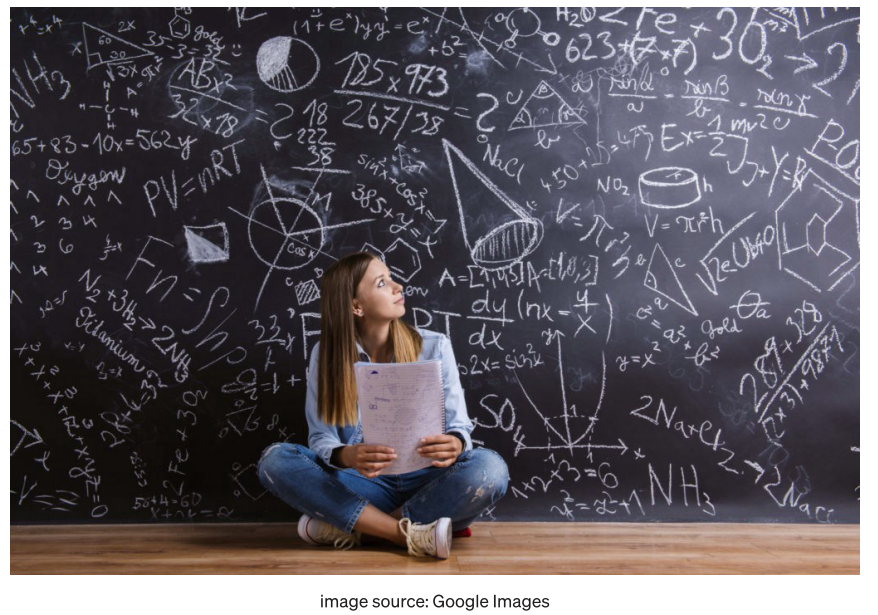
\includegraphics[width=0.8\linewidth,keepaspectratio]{qmaths}
\end{center}

\tiny{(Ref: Beginner’s Guide to Quantum Computing Literature \& Notation - Abby Mitchell)}

\end{frame}


%%%%%%%%%%%%%%%%%%%%%%%%%%%%%%%%%%%%%%%%%%%%%%%%%%%%%%%%%%%
 \begin{frame}[fragile]\frametitle{Representing Qubits using Vectors}
\begin{itemize}
\item Qubits can be represented mathematically as vectors
(specifically state-vectors)
\item Can operate on quantum states (state-vectors) using gates (matrices).
\item All this does is convert one state vector to
another state vector.
\item This is just like geometric transmigrations of points.
\end{itemize}


\tiny{(Ref: Beginner’s Guide to Quantum Computing Literature \& Notation - Abby Mitchell)}

\end{frame}

%%%%%%%%%%%%%%%%%%%%%%%%%%%%%%%%%%%%%%%%%%%%%%%%%%%%%%%%%%%
 \begin{frame}[fragile]\frametitle{Representing Qubits using Vectors}
\begin{itemize}
\item $ \ket 0 $ represents a vector, a qubit state that will collapse to $0$
\item $ \ket 1 $ represents a vector, a qubit state that will collapse to $1$
\end{itemize}

\begin{center}
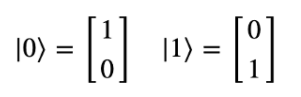
\includegraphics[width=0.3\linewidth,keepaspectratio]{qmaths4}
\end{center}


\tiny{(Ref: Beginner’s Guide to Quantum Computing Literature \& Notation - Abby Mitchell)}

\end{frame}


%%%%%%%%%%%%%%%%%%%%%%%%%%%%%%%%%%%%%%%%%%%%%%%%%%%%%%%%%%%
 \begin{frame}[fragile]\frametitle{Orthonormal Bases}
\begin{itemize}
\item A ‘basis' is a set of vectors in a given geometrical area (vector
space) for which all possible vectors in that space can be represented.
\item 'Computational Basis', 'Z-basis' with $ \ket 0 $ and $ \ket 1 $ basis vectors, can be used to linearly combine to compose any vector.
\item Orthogonal: vectors $ \ket 0 $  and $ \ket 1 $  are perpendicular to each other

\item Orthonormal: vectors $ \ket 0 $  and $ \ket 1 $  are at right angles to each other plus both are unit vectors.
\end{itemize}

\begin{center}
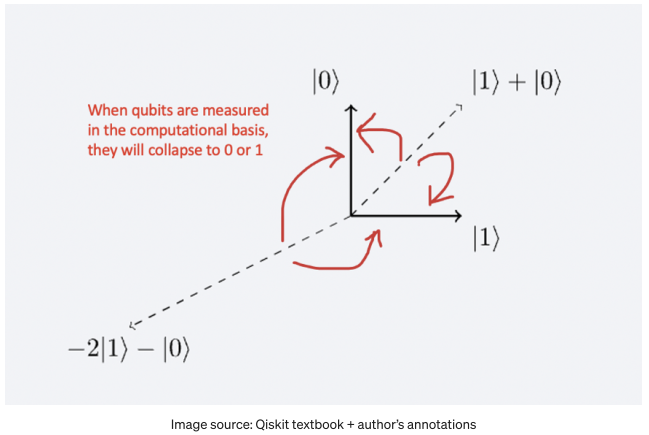
\includegraphics[width=0.5\linewidth,keepaspectratio]{qmaths5}
\end{center}


\tiny{(Ref: Beginner’s Guide to Quantum Computing Literature \& Notation - Abby Mitchell)}

\end{frame}

%%%%%%%%%%%%%%%%%%%%%%%%%%%%%%%%%%%%%%%%%%%%%%%%%%%%%%%%%%%
 \begin{frame}[fragile]\frametitle{$\ket {Dirac Notation} $}
\begin{itemize}
\item $ \bra {} $ is a bra and $\ket {} $ is a ket.
\item Basis ‘Ket’ vectors can represent any vector within our vector space which is called the Hilbert space, this space is where all possible states of our qubits ‘live’.
\item Bra is a vector which is the adjoint of the vector inside it. The adjoint or conjugate transpose, is just a fancy mathematical word for a new vector where the rows and columns are switched, and the values within the vector are conjugated.
\end{itemize}

\begin{center}
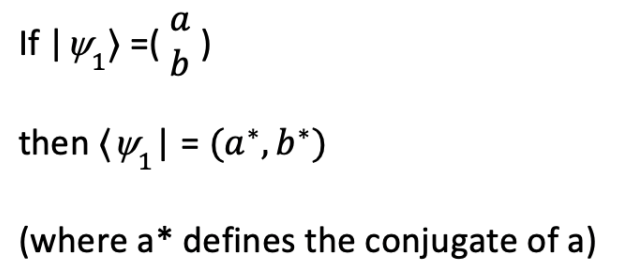
\includegraphics[width=0.3\linewidth,keepaspectratio]{qmaths6}
\end{center}



\tiny{(Ref: Beginner’s Guide to Quantum Computing Literature \& Notation - Abby Mitchell)}

\end{frame}

%%%%%%%%%%%%%%%%%%%%%%%%%%%%%%%%%%%%%%%%%%%%%%%%%%%%%%%%%%%
 \begin{frame}[fragile]\frametitle{$\ket {Dirac Notation} $}
\begin{itemize}
\item The Bra-Ket of two vectors is called the scalar product, and is noted as: $\braket {\psi_a} {\psi_b}$

\item For example, the probability of measuring a random quantum state $\ket \psi $ and finding it in the $\ket 0 $  basis state is equal to the absolute square of their scalar product or their Bra-Ket. Its a projection on $\ket 0 $, an overlap.

\begin{center}
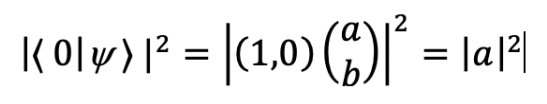
\includegraphics[width=0.4\linewidth,keepaspectratio]{qmaths7}
\end{center}

\item Gates are matrices, and we can apply them to our quantum states.For example, $X \ket \psi $ is the $X$ gate (formally referred to as the Pauli-X gate) applied to our quantum state $X \ket \psi $. 

\begin{center}
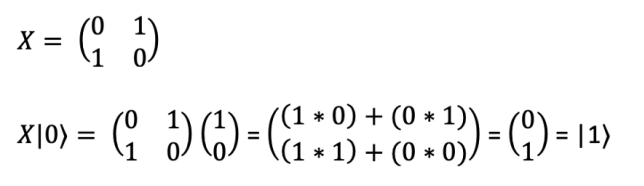
\includegraphics[width=0.7\linewidth,keepaspectratio]{qmaths8}
\end{center}

\end{itemize}




\tiny{(Ref: Beginner’s Guide to Quantum Computing Literature \& Notation - Abby Mitchell)}

\end{frame}

%%%%%%%%%%%%%%%%%%%%%%%%%%%%%%%%%%%%%%%%%%%%%%%%%%%%%%%%%%%
 \begin{frame}[fragile]\frametitle{$\ket {Dirac Notation} $}
\begin{itemize}
\item A general gate, called an ‘operator’,write it as $U$, and apply it to
some qubit state $\ket \psi$ then eigen model will have : $U \ket \psi = u \ket {\psi'}$, where $u$ is eigenvalue and the state $\ket {\psi'}$ its corresponding eigen vector.

\item Hamiltonian is a general example of an
Operator that acts upon Quantum state $\ket \psi$  to give  Quantum state’s
corresponding energy Eigenvalues and Eigenvectors as follows: $H \ket \psi = E \ket {\psi_i}$ 
\item The
energy Eigenvalues are also known as Observables and represent the actual
energy of the corresponding Eigenvector.

\item The Hamiltonian is a ‘Unitary’ operator, meaning that the Matrix that
represents the operator has the mathematical characteristic that its inverse
is its Conjugate Transpose: i.e. U is Unitary if $U^*U = UU^* = I$

\item  Quantum gates such as the Hadamard gate ($H$) and the C-not gate ($CX$), which we can use in quantum computing, are unitary. This
essentially means they are reversible i.e. $H \ket \psi H^* = I \ket \psi $
\end{itemize}




\tiny{(Ref: Beginner’s Guide to Quantum Computing Literature \& Notation - Abby Mitchell)}

\end{frame}

%%%%%%%%%%%%%%%%%%%%%%%%%%%%%%%%%%%%%%%%%%%%%%%%%%%%%%%%%%%
 \begin{frame}[fragile]\frametitle{Common Mathematical Notation}

\begin{center}
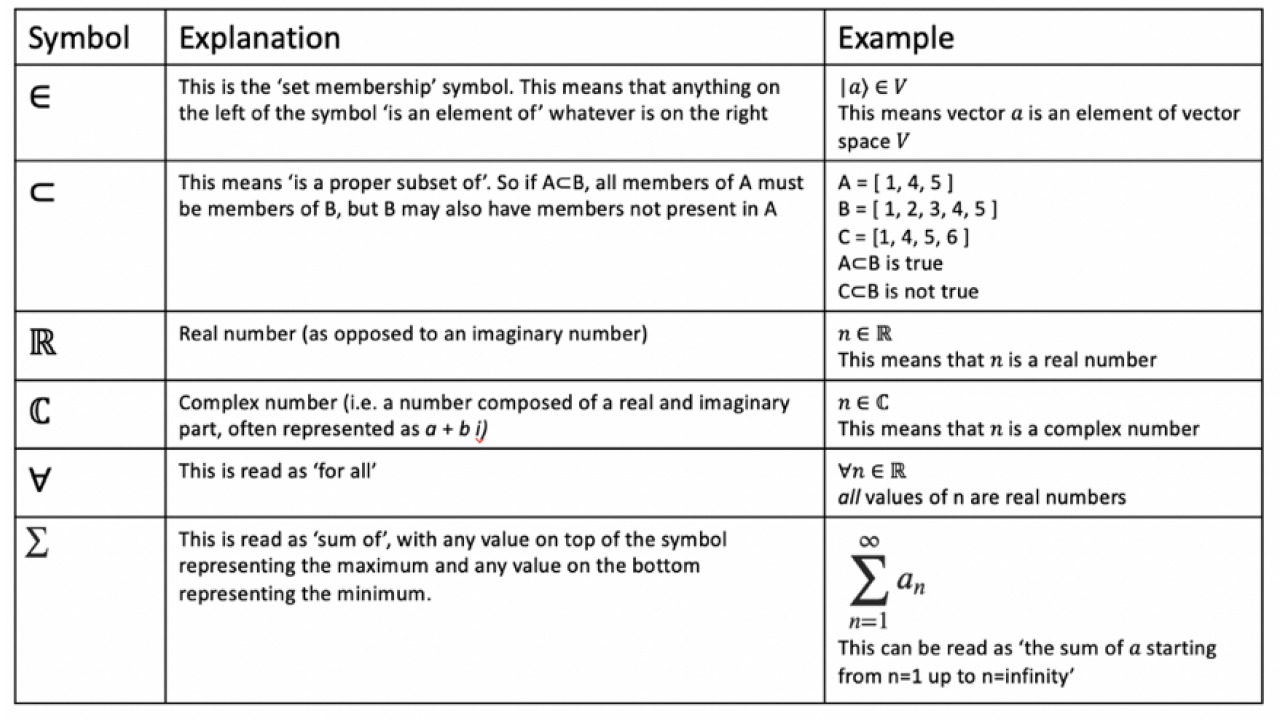
\includegraphics[width=0.8\linewidth,keepaspectratio]{qmaths1}
\end{center}

\tiny{(Ref: Beginner’s Guide to Quantum Computing Literature \& Notation - Abby Mitchell)}

\end{frame}

%%%%%%%%%%%%%%%%%%%%%%%%%%%%%%%%%%%%%%%%%%%%%%%%%%%%%%%%%%%
 \begin{frame}[fragile]\frametitle{Common Vector Notation in Quantum}

\begin{center}
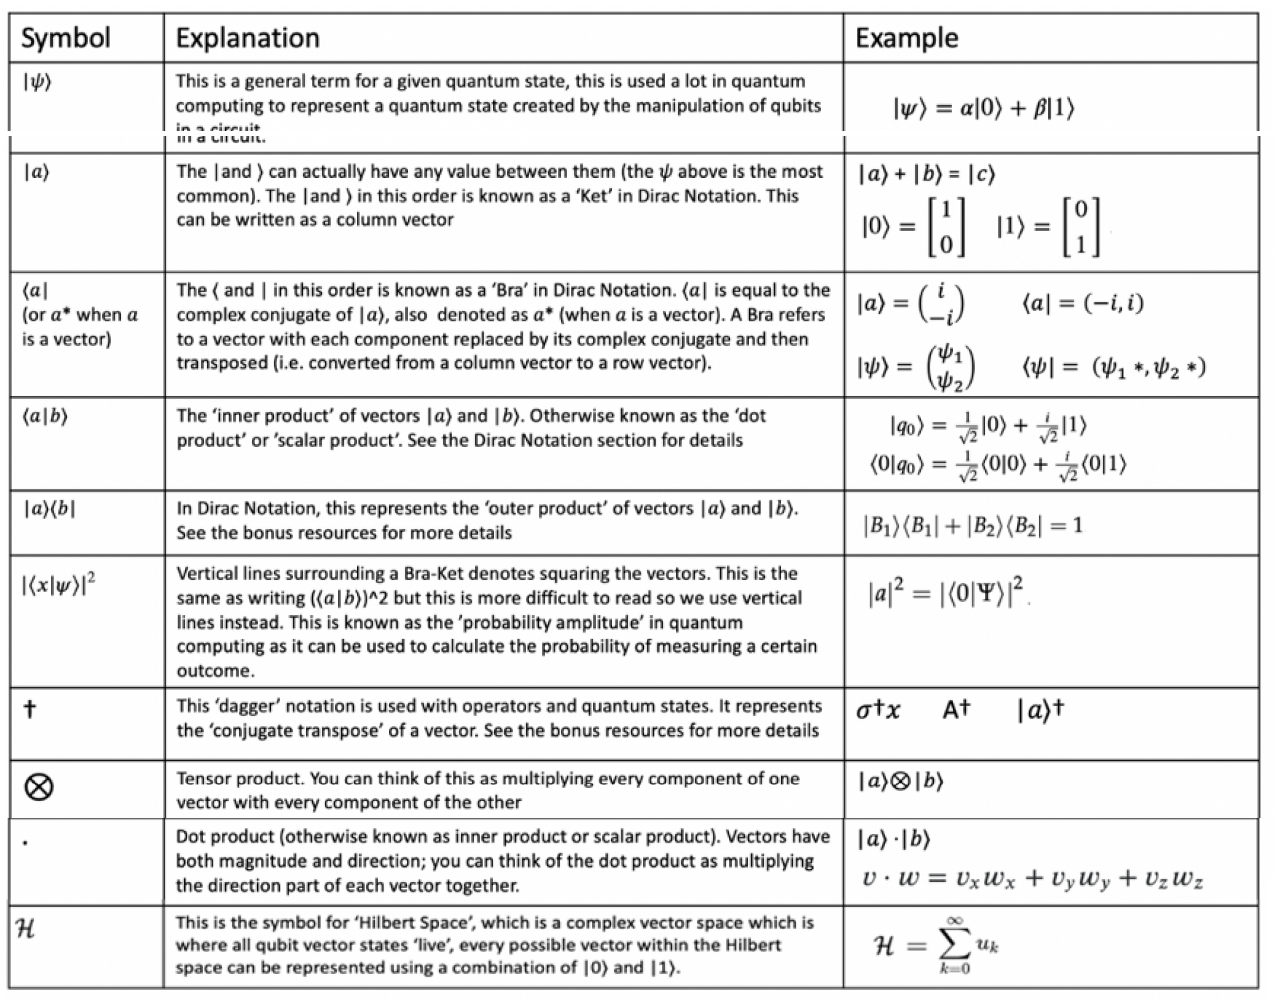
\includegraphics[width=0.8\linewidth,keepaspectratio]{qmaths2}
\end{center}

\tiny{(Ref: Beginner’s Guide to Quantum Computing Literature \& Notation - Abby Mitchell)}

\end{frame}

%%%%%%%%%%%%%%%%%%%%%%%%%%%%%%%%%%%%%%%%%%%%%%%%%%%%%%%%%%%
 \begin{frame}[fragile]\frametitle{Common Quantum Operators}

\begin{center}
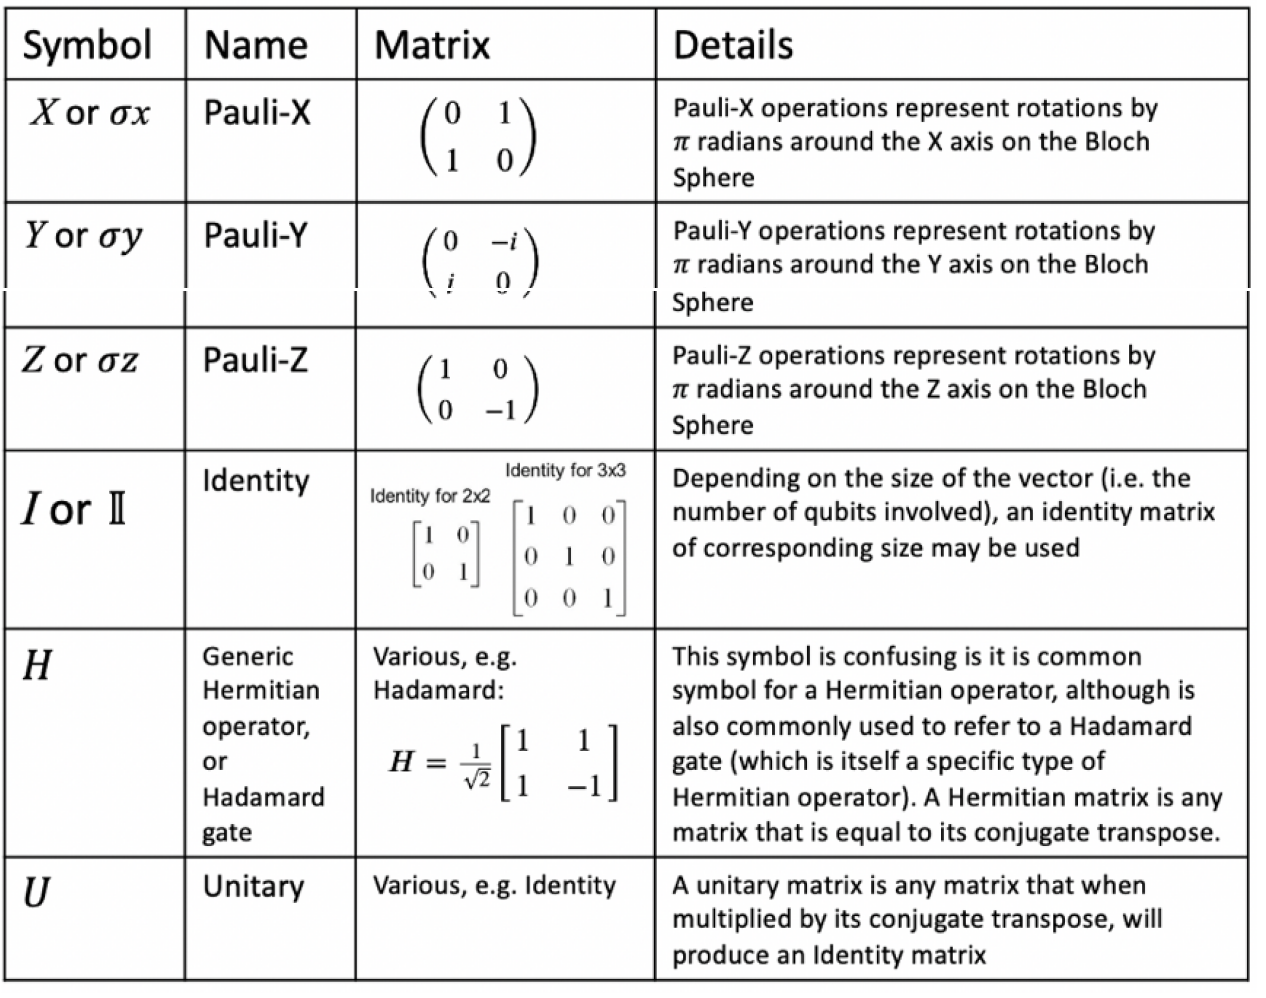
\includegraphics[width=0.8\linewidth,keepaspectratio]{qmaths3}
\end{center}

\tiny{(Ref: Beginner’s Guide to Quantum Computing Literature \& Notation - Abby Mitchell)}

\end{frame}


% %%%%%%%%%%%%%%%%%%%%%%%%%%%%%%%%%%%%%%%%%%%%%%%%%%%%%%%%%%%
 % \begin{frame}[fragile]\frametitle{Brief overview}
% \begin{itemize}
	% \item Hilbert spaces and quantum mechanics.
	% \item Tensor products and entangled quantum states.
	% \item Quantum bits (qubits), the physics of computation, elements of quantum computing.
	% \item Tractability of computation (e.g., factoring and NP/NP-complete problems).
	% \item Theoretical models for quantum computing.
	% \item Suggestions for practical implementations of quantum computers.
	% \item Problems and prospects.
% \end{itemize}

% \end{frame}

% %%%%%%%%%%%%%%%%%%%%%%%%%%%%%%%%%%%%%%%%%%%%%%%%%%%%%%%%%%%
 % \begin{frame}[fragile]\frametitle{Some History}
% \begin{itemize}
	% \item Physics
	% \item Philosophy (theory of knowledge)
	% \item Mathematics
	% \begin{enumerate}
		% \item Matrix manipulation
		% \item Topology
		% \item Algebra
		% \item Lie groups
		% \item Manifolds and relativity theory
		% \item Algebraic topology
	% \end{enumerate}
% \end{itemize}

% \end{frame}


%%%%%%%%%%%%%%%%%%%%%%%%%%%%%%%%%%%%%%%%%%%%%%%%%%%%%%%%%%%
 \begin{frame}[fragile]\frametitle{Hilbert space setting for quantum mechanics}

\begin{itemize}
	\item A Hilbert space $\hilbert$ is a complete normed vector space over $\complex$ :
	\begin{enumerate}
		\item $\hilbert$ is a vector space over $\complex$
		\item There is an inner product \newline
			$\braket \cdot \cdot$ : $\hilbert$ x $\hilbert \rightarrow \complex$
			\newline
			which is conjugate linear: \newline
			$\braket v w = \overline{\braket w v} $  \newline
			$\braket {\alpha v} w = \alpha \braket v w $
				for $\alpha \in \complex$ \newline
			$\braket {v+w} z = \braket v z + \braket w z $ \newline
			$\braket vv \ge 0$ \newline
			and \newline
			$\braket vv = 0$ iff $v = 0$
		\item From the inner product, as usual, we define the norm of a vector: \newline
			$ \Vert v \Vert ^ 2 = \braket v v $
		\item $\hilbert$ is complete with respect to the norm.
	\end{enumerate}
	
\end{itemize}

\tiny{(Ref: A brief overview of quantum computing - Tom Carter)}

\end{frame}

%%%%%%%%%%%%%%%%%%%%%%%%%%%%%%%%%%%%%%%%%%%%%%%%%%%%%%%%%%%
 \begin{frame}[fragile]\frametitle{Bra Ket notation}

\begin{itemize}
	\item We will typically use the bra/ket notation: \newline
		$ \ket v $ is a vector in $\hilbert$, and \newline
		$ \bra v $ is the covector which is the conjugate transpose of v. \newline
		This notation also allows us to represent the outer product of a vector and
		covector as $\ket v \bra w$, which, for example, acts on a vector $\ket z$
		as $\ket v \braket w z$.
		 For example, if \{$v_1$,$v_2$\} is an orthonormal basis for a two-dimensional
		  Hilbert space, $\ket {v_1}\bra {v_2}$ is the transformation
			that maps $\ket {v_2}$ to $\ket {v_1}$ and $\ket {v_1}$ to $\tcol 00$ since
			$$\begin{array}{l}
			\ket {v_1}\bra {v_2}\ket {v_2} = \ket {v_1}\braket {v_2}{v_2} = \ket {v_1}\\
			\ket {v_1}\bra {v_2}\ket {v_1} = \ket {v_1}\braket {v_2}{v_1} = 0 \ket {v_1} = \col 00.\\
  			\end{array}$$
			Equivalently, $\ket {v_1}\bra {v_2}$ can be written in matrix form where
			$\ket {v_1} = \tcol 10$, $\bra {v_1} = (1, 0)$, $\ket {v_2} = \tcol 01$,
			 and $\bra {v_2} = (0, 1)$.
			Then 
			$$\ket {v_1}\bra {v_2} = \col 10 (0, 1) = 
					\left(\begin{array}{cc}0&1\\0&0\end{array}\right).$$
	\end{itemize}
	
\tiny{(Ref: A brief overview of quantum computing - Tom Carter)}
	
\end{frame}

%%%%%%%%%%%%%%%%%%%%%%%%%%%%%%%%%%%%%%%%%%%%%%%%%%%%%%%%%%%
 \begin{frame}[fragile]\frametitle{Bra Ket notation}

	\begin{itemize}		
	\item A unitary operator $ U : \hilbert \to \hilbert $ is a linear mapping
		whose conjugate transpose is its inverse:  $ U^\dag = U^{-1} $
	\item Unitary operators are norm preserving: \newline
		$ \bra v U^\dag U \ket v = \braket v v = \Vert v \Vert ^2 $
	\item We will think of a quantum state as a (normalized) vector $ \ket v \in \hilbert $,
		where we think of $\braket v v$ as the probability of observing the state.
		For math folks, we are in effect working in Complex projective space, normalizing
		to 1 so that the probabilities make sense.
	\item The dynamical evolution of a quantum system is expressed as a unitary operator acting on
		the quantum state.  Note that probabilities are preserved.
\end{itemize}

\tiny{(Ref: A brief overview of quantum computing - Tom Carter)}

\end{frame}

%%%%%%%%%%%%%%%%%%%%%%%%%%%%%%%%%%%%%%%%%%%%%%%%%%%%%%%%%%%
 \begin{frame}[fragile]\frametitle{Eigenvalues}

\begin{itemize}
	\item Eigenvalues of a unitary matrix are of the form $ e ^ {i\omega} $ where $\omega$ is a
		real-valued angle.  A unitary operator is in effect a rotation.
	\item In the Schr\"odinger equation, $U$ is determined by the {\em Hamiltonian} or
		energy operator $H$ via $U = e^{iHt}$.
	\item A measurement consists of applying an operator $O$ to a quantum state $v$.  To
		correspond to a classical observable, $O$ must be {\em Hermitian}, $O^\dag = O$, so
		that all its eigenvalues are real.  If one of its eigenvalues $\lambda$ is associated with
		a single eigenvector $u_\lambda$, then we observe the value $\lambda$ with probability
		$\vert \braket v {u_\lambda} \vert ^ 2$ (i.e., the square of the length of
		the projection along $u_\lambda$).
\end{itemize}

\tiny{(Ref: A brief overview of quantum computing - Tom Carter)}

\end{frame}

%%%%%%%%%%%%%%%%%%%%%%%%%%%%%%%%%%%%%%%%%%%%%%%%%%%%%%%%%%%
 \begin{frame}[fragile]\frametitle{Eigenvalues}

\begin{itemize}
	\item In general, if there is more than one eigenvector $u_\lambda$ associated with the
		eigenvalue $\lambda$, we let $P_\lambda$ be the projection operator onto the subspace
		spanned by the eigenvectors, and the probability of observing $\lambda$ when the
		system is in state $v$ is $\Vert v P_\lambda \Vert ^ 2 $.
		
	\item Most projection operators do not commute with each other, and are not invertible.
	  	Therefore, we can expect that the order in which we do measurements will matter, and that
	   	doing a measurement will irreversibly change the state of the quantum system.

\end{itemize}

\tiny{(Ref: A brief overview of quantum computing - Tom Carter)}

\end{frame}

%%%%%%%%%%%%%%%%%%%%%%%%%%%%%%%%%%%%%%%%%%%%%%%%%%%%%%%%%%%
 \begin{frame}[fragile]\frametitle{Tensor products}

\begin{itemize}
	\item Tensor products \newline
	We can form tensor products of a wide variety of objects.  For example: 
	\begin{enumerate}
		\item The tensor product of an $n$ dimensional vector $u$ and a $k$ dimensional vector $v$ is 				an $nk$ dimensional vector $u \tensor v$.
		\item If $A$ and $B$ are operators on $n$ and $k$ dimensional vectors, respectively, then $A \tensor B$ is an operator on $nk$ dimensional vectors.
		\item if $\hilbert_1$ and $\hilbert_2$ are Hilbert spaces, then $\hilbert_1 \tensor \hilbert_2$ is also a Hilbert space.  If $\hilbert_1$ and $\hilbert_2$ are finite dimensional with bases $\{u_1, u_2, \ldots u_n\}$ and $\{v_1, v_2, \ldots v_m\}$ respectively, then $\hilbert_1 \tensor \hilbert_2$ has dimension $nm$ with basis $\{u_i \tensor v_j | 1 \le i \le n, 1 \le j \le m\}$.
\end{enumerate}
\end{itemize}

\tiny{(Ref: A brief overview of quantum computing - Tom Carter)}

\end{frame}

%%%%%%%%%%%%%%%%%%%%%%%%%%%%%%%%%%%%%%%%%%%%%%%%%%%%%%%%%%%
 \begin{frame}[fragile]\frametitle{Tensor products}

\begin{itemize}
		\item Tensor products obey a number of nice rules, such as:
		For matrices $A$, $B$, $C$, $D$, $U$, vectors $u$, $v$, $w$, and scalars $a$, $b$, $c$, $d$ the following hold:

\begin{eqnarray*}
(A \tensor B) (C \tensor D) &=& AC\tensor BD\\
(A \tensor B) (u \tensor v) &=& Au\tensor Bv\\
(u+v)\tensor w&=& u\tensor w + v\tensor w\\
u\tensor(v+w)&=& u\tensor v + u\tensor w\\
au\tensor bv &=& ab(u\tensor v)
\end{eqnarray*}

Thus for matrices,
$$\left(\begin{array}{cc}A & B\\C & D\end{array}\right) \tensor U = 
\left(\begin{array}{cc}A \tensor U & B \tensor U\\C \tensor U & D \tensor U\end{array}\right),$$

which specializes for scalars to
$$\left(\begin{array}{cc}a & b\\c & d\end{array}\right) \tensor U = 
\left(\begin{array}{cc}a U & b U\\c U & d U\end{array}\right).$$

\end{itemize}

\tiny{(Ref: A brief overview of quantum computing - Tom Carter)}

\end{frame}

%%%%%%%%%%%%%%%%%%%%%%%%%%%%%%%%%%%%%%%%%%%%%%%%%%%%%%%%%%%
 \begin{frame}[fragile]\frametitle{Tensor products}

\begin{itemize}

	\item The conjugate transpose distributes over tensor products, i.e.
$$(A\tensor B)^\dag= A^\dag\tensor B^\dag.$$

	\item The tensor product of several matrices is unitary if and only if each one of the
matrices is unitary up to a constant.  Let $U = A_1\tensor \dots \tensor A_n$.  Then
$U$ is unitary if $A_i^\dag A_i = k_i I$ and $\prod_ik_i = 1$.
\begin{eqnarray*}U^\dag U &=& (A_1^\dag\tensor \dots \tensor A_n^\dag )(A_1\tensor \dots \tensor A_n)\\
&=& A_1^\dag A_1\tensor \dots \tensor A_n^\dag A_n\\
&=& k_1I\tensor \dots \tensor k_nI\\
&=& I\\
\end{eqnarray*}

\end{itemize}

\tiny{(Ref: A brief overview of quantum computing - Tom Carter)}

\end{frame}

%%%%%%%%%%%%%%%%%%%%%%%%%%%%%%%%%%%%%%%%%%%%%%%%%%%%%%%%%%%
 \begin{frame}[fragile]\frametitle{Tensor products}

\begin{itemize}
	\item Note that $\braket {u \tensor v} {w \tensor z} = \braket uw \braket vz$.  
	This implies that $\braket {0 \tensor u} {0 \tensor u} = 0$, and therefore $0 \tensor u$ must
	be the zero vector of the tensor product Hilbert space.
	
	This in turn implies (reminds us?) that the tensor product space is actually the equivalence
	classes in a quotient space.
	
	In particular, if $A$ and $B$ are vector spaces, $F$ is the free abelian group on $A\times B$,
	and $K$ is the subgroup of $F$ generated by all elements of the following forms (where \newline	
	$a, a_1, a_2\in A, b, b_1, b_2\in B, \alpha$ a scalar):
	\begin{enumerate}
		\item $(a_1 + a_2,b) - (a_1,b) - (a_2,b)$
		\item $(a,b_1 + b_2) - (a,b_1) - (a,b_2)$
		\item $(\alpha a,b) - (a,\alpha b)$
	\end{enumerate}
	then $A\tensor B$ is the quotient space $F/K$.
	 
\end{itemize}

\tiny{(Ref: A brief overview of quantum computing - Tom Carter)}

\end{frame}

%%%%%%%%%%%%%%%%%%%%%%%%%%%%%%%%%%%%%%%%%%%%%%%%%%%%%%%%%%%
 \begin{frame}[fragile]\frametitle{Qubits}

\begin{itemize}
	\item A quantum bit, or qubit\index{qubit}, is a unit vector in a two dimensional
complex vector space for which a particular orthonormal basis, denoted by
$\{\ket 0, \ket 1\}$, 
has been fixed. It is important to notice that the basis vector $\ket 0$ is NOT the zero vector of the vector space.
\item The orthonormal basis
$\ket 0$ and $\ket 1$ may correspond to the $\ket{\uparrow}$ and 
$\ket{\to}$ polarizations of a photon respectively, or to the polarizations
$\ket{\nearrow}$ and $\ket{\nwarrow}$. Or $\ket 0$ and $\ket 1$ could 
correspond to the spin-up and spin-down states ($\ket{\uparrow}$ and $\ket{\downarrow}$) of an electron.
\end{itemize}

\tiny{(Ref: A brief overview of quantum computing - Tom Carter)}

\end{frame}

%%%%%%%%%%%%%%%%%%%%%%%%%%%%%%%%%%%%%%%%%%%%%%%%%%%%%%%%%%%
 \begin{frame}[fragile]\frametitle{Qubits}

\begin{itemize}

\item For the purposes of quantum computing, the basis states $\ket 0$ and $\ket 1$ 
are taken to encode the classical bit values
$0$ and $1$ respectively. 
Unlike classical bits however, qubits can be in a superposition of
$\ket 0$ and $\ket 1$ such as $a\ket 0 + b\ket 1$
where $a$ and $b$ are complex numbers such that 
$\vert a\vert^2 + \vert b\vert^2 = 1$. If such a superposition is measured with
respect to the basis $\{\ket 0,\ket 1\}$, the probability that the 
measured value is $\ket 0$ is $\vert a\vert ^2$ and the probability that the
measured value is $\ket 1$ is  $\vert b\vert ^2$.

\end{itemize}

\tiny{(Ref: A brief overview of quantum computing - Tom Carter)}

\end{frame}


%%%%%%%%%%%%%%%%%%%%%%%%%%%%%%%%%%%%%%%%%%%%%%%%%%%%%%%%%%%
 \begin{frame}[fragile]\frametitle{Qubits}

\begin{itemize}

\item Key properties of quantum bits:
 \begin{enumerate}
 \item A qubit can be in a superposition\index{superposition} state of $0$ and $1$.  
 \item Measurement of a qubit in a superposition state will yield
 probabilistic results.
 \item Measurement of a qubit changes the state to the one measured.
 \item Qubits cannot be copied exactly.  This is known as the `no cloning' principle.  Interestingly, it is nonetheless possible to `teleport' a quantum state, but in the process, the original quantum state is destroyed \ldots
 \end{enumerate}

\end{itemize}

\tiny{(Ref: A brief overview of quantum computing - Tom Carter)}

\end{frame}

%%%%%%%%%%%%%%%%%%%%%%%%%%%%%%%%%%%%%%%%%%%%%%%%%%%%%%%%%%%
 \begin{frame}[fragile]\frametitle{Qubits}

\begin{itemize}
	\item If we have available more than one (physical) qubit, we may be able to {\em entangle} them.  The tensor product of the Hilbert spaces for the individual qubits is the appropriate model for these entangled systems.

	\item For example, if we have two qubits with bases $\{\ket 0_1,\ket 1_1\}$ and
	$\{ \ket 0_2,\ket 1_2\}$ respectively, the tensor product space has the basis 
	$$\{\ket 0_1\tensor\ket 0_2,\ket 0_1\tensor\ket 1_2,\ket 1_1\tensor\ket 0_2,\ket 1_1\tensor\ket 1_2\}.$$  We can (conveniently) denote this basis as
$$\{\ket{00},\ket{01},\ket{10},\ket{11}\}.$$
\end{itemize}

\tiny{(Ref: A brief overview of quantum computing - Tom Carter)}

\end{frame}

%%%%%%%%%%%%%%%%%%%%%%%%%%%%%%%%%%%%%%%%%%%%%%%%%%%%%%%%%%%
 \begin{frame}[fragile]\frametitle{Qubits}

\begin{itemize}

	\item More generally, if we have $n$ qubits to which we can apply common measurements, we will be working in the $2^n$-dimensional Hilbert space with basis
$$\{\ket{00\ldots00},\ket{00\ldots01},\ldots,\ket{11\ldots10},\ket{11\ldots11}\}$$
\item A typical quantum state for an $n$-qubit system is
$$\sum_{i = 0}^{2^n-1}a_i\ket i$$
where $a_i\in\complex$, and $\{\ket i\}$ is the basis, with (in our notation) $i$ written as an $n$-bit binary number.

\end{itemize}

\tiny{(Ref: A brief overview of quantum computing - Tom Carter)}

\end{frame}

%%%%%%%%%%%%%%%%%%%%%%%%%%%%%%%%%%%%%%%%%%%%%%%%%%%%%%%%%%%
 \begin{frame}[fragile]\frametitle{Qubits}

\begin{itemize}
\item A classical (macroscopic) physical 
object broken into pieces can be described and measured as separate components.
An $n$-particle quantum system cannot always be
described in terms of the states of its component pieces. For instance, 
the state \newline$\ket{00}+\ket{11}$ cannot be decomposed into separate states
of each of the two qubits.  In other words, we cannot find 
$a_1,a_2,b_1,b_2$ such that 
$$(a_1\ket 0 + b_1\ket 1)\tensor (a_2\ket 0 + b_2\ket 1) = \ket{00}+\ket{11}$$
since 
$$(a_1\ket 0 + b_1\ket 1)\tensor (a_2\ket 0 + b_2\ket 1) = $$
$$  a_1a_2\ket{00} + a_1b_2\ket{01} + b_1a_2\ket{10} + b_1b_2\ket{11}$$ and
$a_1b_2 = 0$ implies that either $a_1a_2 = 0$ or $b_1b_2 = 0$.
States which cannot be decomposed in this way are called entangled\index{entangled} states.
These are states that don't have classical counterparts, and
for which our intuition is likely to fail.

\end{itemize}

\tiny{(Ref: A brief overview of quantum computing - Tom Carter)}

\end{frame}

%%%%%%%%%%%%%%%%%%%%%%%%%%%%%%%%%%%%%%%%%%%%%%%%%%%%%%%%%%%
 \begin{frame}[fragile]\frametitle{Qubits}

\begin{itemize}
\item Particles are entangled if a measurement of one
affects a measurement of the other. For example, the state 
$\frac{1}{\sqrt{2}}(\ket{00}+\ket{11})$ is entangled since the 
probability of measuring the first bit as $\ket 0$ is $1/2$ 
if the second bit has not been measured. However, if the second bit
has been measured, the probability that the first bit is 
measured as $\ket 0$ is either $1$ or $0$, depending on whether the
second bit was measured as $\ket 0$ or $\ket 1$, respectively. On the other hand, the state
$\frac{1}{\sqrt{2}}(\ket{00}+\ket{01})$ is not entangled. Since 
$\frac{1}{\sqrt{2}}(\ket{00}+\ket{01}) = \ket 0\tensor \frac{1}{\sqrt{2}}(\ket{0}+\ket{1})$, any 
measurement of the first bit will yield $\ket 0$ regardless of
measurements of the second bit.  Similarly, the second bit has a 
fifty-fifty chance of being measured as $\ket 0$ regardless of 
measurements of the first bit. Note that entanglement in terms of particle measurement dependence is equivalent to the definition of entangled
states as states that cannot be written as a tensor product of individual
states.
\end{itemize}

\tiny{(Ref: A brief overview of quantum computing - Tom Carter)}

\end{frame}

%%%%%%%%%%%%%%%%%%%%%%%%%%%%%%%%%%%%%%%%%%%%%%%%%%%%%%%%%%%
 \begin{frame}[fragile]\frametitle{Quantum Computing}

\begin{itemize}

	\item This exponential growth in number of states, together with the ability to subject the entire space to transformations (either unitary dynamical evolution of the system, or a measurement projection into an eigenvector subspace), provides the foundation for quantum computing.
	\item An interesting (apparent) dilemma is the energetic costs/irreversability of classical computing.  Since unitary transformations are invertible, quantum computations (except measurements) will all be reversible.  The classical boolean operations such as $b_1\land b_2$, $b_1\lor b_2$, and $b_1\lnandb b_2$ are irreversible, and therefore cannot directly be used as basic operations for quantum computers.

\end{itemize}

\tiny{(Ref: A brief overview of quantum computing - Tom Carter)}

\end{frame}

%%%%%%%%%%%%%%%%%%%%%%%%%%%%%%%%%%%%%%%%%%%%%%%%%%%%%%%%%%%
 \begin{frame}[fragile]\frametitle{Quantum Computing}

\begin{itemize}

	\item The logical nand-gate ($b_1\lnandc b_2$) is sufficient to generate all the traditional boolean functions (e.g., $\sim\negmedspace b \equiv b\ \lnanda b$).  We will look for simple quantum gates that are similarly generic for quantum operations.
\end{itemize}

\tiny{(Ref: A brief overview of quantum computing - Tom Carter)}

\end{frame}

%%%%%%%%%%%%%%%%%%%%%%%%%%%%%%%%%%%%%%%%%%%%%%%%%%%%%%%%%%%
 \begin{frame}[fragile]\frametitle{Simple quantum gates}

\begin{itemize}
	\item  These are some examples of useful single-qubit quantum state transformations.
Because of linearity, the transformations are fully specified by
their effect on the basis vectors. 
The associated matrix is also shown.
$$\begin{array}{ll}
\begin{array}{lrcl}
I\ :& \ket{0} & \to & \ket{0}\\
  & \ket{1} & \to & \ket{1}\\
\end{array} &
\left(\begin{array}{cc}1 & 0\\ 0 & 1\end{array}\right)\\
\begin{array}{lrcl}
X:& \ket{0} & \to & \ket{1}\\
  & \ket{1} & \to & \ket{0}\\
\end{array} &
\left(\begin{array}{cc}0 & 1\\ 1 & 0\end{array}\right)\\
\begin{array}{lrcl}
Y:& \ket{0} & \to & \ket{1}\\
  & \ket{1} & \to &-\ket{0}\\
\end{array} &
\left(\begin{array}{cc}0 & -1\\ 1 & 0\end{array}\right)\\
\begin{array}{lrcl}
Z:& \ket{0} & \to & \ket{0}\\
  & \ket{1} & \to & -\ket{1}\\
\end{array} &
\left(\begin{array}{cc}1 & 0\\ 0 & -1\end{array}\right)\\
\end{array}$$ 
$I$ is the identity transformation, $X$ is negation, $Z$ is
a phase shift operation, and $Y = ZX$ is a combination of both.  
All these gates are unitary.  For example
$$YY^* = \left(\begin{array}{cc}0 & -1\\ 1 & 0\end{array}\right) 
	 \left(\begin{array}{cc}0 & 1\\ -1 & 0\end{array}\right) = I.$$


\end{itemize}

\tiny{(Ref: A brief overview of quantum computing - Tom Carter)}

\end{frame}

%%%%%%%%%%%%%%%%%%%%%%%%%%%%%%%%%%%%%%%%%%%%%%%%%%%%%%%%%%%
 \begin{frame}[fragile]\frametitle{Simple quantum gates}

\begin{itemize}

\item Probably the most important gate is the controlled-{\sc not} gate, $C_{not}$, which
operates on two qubits as follows: it changes the second 
bit if the first bit is $1$ and leaves the bit unchanged otherwise.
$$\begin{array}{ll}\begin{array}{lrcl}
C_{not}:& \ket{00} & \to & \ket{00}\\
        & \ket{01} & \to & \ket{01}\\
        & \ket{10} & \to & \ket{11}\\
        & \ket{11} & \to & \ket{10}\\
\end{array} & \left(\begin{array}{cccc}1 & 0 & 0 & 0\\ 0 & 1 & 0 & 0\\
				       0 & 0 & 0 & 1\\ 0 & 0 & 1 & 0\end{array}\right)\\
\end{array}$$
The transformation $C_{not}$ is unitary since $C_{not}^*=C_{not}$ and
$C_{not}C_{not}= I$. 
The $C_{not}$ gate cannot
be decomposed into a tensor product of two 
single-bit transformations.

\end{itemize}

\tiny{(Ref: A brief overview of quantum computing - Tom Carter)}

\end{frame}

%%%%%%%%%%%%%%%%%%%%%%%%%%%%%%%%%%%%%%%%%%%%%%%%%%%%%%%%%%%
 \begin{frame}[fragile]\frametitle{Tractability of computation}

\begin{itemize}
	\item Creativity and Art
	\begin{enumerate}
		\item Knowing when to pattern
		\item Symbol attachment and creation; \newline 
			patterns/symbols as revealers and \newline
			concealers
		\item Levels of patterning
	\end{enumerate}
	\item Multiple patterns and selection \newline
		$ (x - 1)(x - 2)(x - 3) - 6 $ \newline
		$ x^3 - 6x^2 + 11x - 12 $ \newline
		$ (x - 4)(x^2 - 2x + 3) $
	\item Adaptive pattern recognition
	\item Are the patterns really there?
\end{itemize}

\tiny{(Ref: A brief overview of quantum computing - Tom Carter)}

\end{frame}

%%%%%%%%%%%%%%%%%%%%%%%%%%%%%%%%%%%%%%%%%%%%%%%%%%%%%%%%%%%
 \begin{frame}[fragile]\frametitle{Map}


We have the map
	$ b_n: \Sigma^2U(n) \rightarrow SU(n+1) $ \newline
given by
	\[ b_n(g, r, s) = \left[ i(g), v_n(r, s) \right] \]
where $i(g)$ is the inclusion,
	$\left[g, h\right] = ghg^{-1}h^{-1}$ \newline
and

$ v_n(r,s) = $

{\small
\[
\left[ \begin{array}{cccccc}
	\alpha & 0 & 0 & \cdots & 0 & \beta (-\overline{\alpha})^0 \\
	\beta (-\overline{\alpha})^0\overline{\beta} &
	   \alpha  &  0  & \cdots & 0 &
	   \beta (-\overline{\alpha})^1 \\
	\beta (-\overline{\alpha})^1\overline{\beta} &
	   \beta (-\overline{\alpha})^0\overline{\beta} &
	   \alpha & \cdots & 0 & \beta (-\overline{\alpha})^2 \\
	\vdots & \vdots & \vdots &  & \vdots & \vdots \\
	\vdots & \vdots & \vdots & \ddots & \vdots & \vdots \\
	\vdots & \vdots & \vdots &  & \vdots & \vdots \\
	\beta (-\overline{\alpha})^{n-1}\overline{\beta} &
	   \beta (-\overline{\alpha})^{n-2}\overline{\beta} &
	   \cdots &  \cdots & \alpha &
	   \beta (-\overline{\alpha})^n \\
	-(-\overline{\alpha})^n\overline{\beta} &
	   -(-\overline{\alpha})^{n-1}\overline{\beta} &
	   \cdots &  \cdots & -(-\overline{\alpha})^0 
	   \overline{\beta} & -(-\overline{\alpha})^n \\
	\end{array} \right]
\]
}

{\small
where
\[ \alpha = \alpha(r,s) =
	\cos(\pi r) + i \sin(\pi r)\cos(\pi s) \]
\[ \beta = \beta(r,s) = i \sin(\pi r)\sin(\pi s) \]
}

\tiny{(Ref: A brief overview of quantum computing - Tom Carter)}

\end{frame}

% %%%%%%%%%%%%%%%%%%%%%%%%%%%%%%%%%%%%%%%%%%%%%%%%%%%%%%%%%%%
 % \begin{frame}[fragile]\frametitle{Map}


% {\tiny
% \begin{verbatim}
% We have the map
	% $ b_n: \Sigma^2U(n) \rightarrow SU(n+1) $ \newline
% given by
	% \[ b_n(g, r, s) = \left[ i(g), v_n(r, s) \right] \]
% where $i(g)$ is the inclusion,
	% $\left[g, h\right] = ghg^{-1}h^{-1}$ \newline
% and

% $ v_n(r,s) = $

% \[
% \left[ \begin{array}{cccccc}
	% \alpha & 0 & 0 & \cdots & 0 & \beta (-\overline{\alpha})^0 \\
	% \beta (-\overline{\alpha})^0\overline{\beta} &
	   % \alpha  &  0  & \cdots & 0 &
	   % \beta (-\overline{\alpha})^1 \\
	% \beta (-\overline{\alpha})^1\overline{\beta} &
	   % \beta (-\overline{\alpha})^0\overline{\beta} &
	   % \alpha & \cdots & 0 & \beta (-\overline{\alpha})^2 \\
	% \vdots & \vdots & \vdots &  & \vdots & \vdots \\
	% \vdots & \vdots & \vdots & \ddots & \vdots & \vdots \\
	% \vdots & \vdots & \vdots &  & \vdots & \vdots \\
	% \beta (-\overline{\alpha})^{n-1}\overline{\beta} &
	   % \beta (-\overline{\alpha})^{n-2}\overline{\beta} &
	   % \cdots &  \cdots & \alpha &
	   % \beta (-\overline{\alpha})^n \\
	% -(-\overline{\alpha})^n\overline{\beta} &
	   % -(-\overline{\alpha})^{n-1}\overline{\beta} &
	   % \cdots &  \cdots & -(-\overline{\alpha})^0 
	   % \overline{\beta} & -(-\overline{\alpha})^n \\
	% \end{array} \right]
% \]
% where
% \[ \alpha = \alpha(r,s) =
	% \cos(\pi r) + i \sin(\pi r)\cos(\pi s) \]
% \[ \beta = \beta(r,s) = i \sin(\pi r)\sin(\pi s) \]

% \end{verbatim}
% }
% \end{frame}